\documentclass[25pt,a0paper,margin=0.5cm,colspace=0.75cm,
               subcolspace=-0.5cm,blockverticalspace=0.75cm]{tikzposter}
\usecolorstyle{Default}
\colorlet{backgroundcolor}{white}

\usepackage[utf8]{inputenc}
\usepackage{amsmath}
\usepackage{amssymb}

% heading-less bibliography (kills the big auto "References" title + its gap)
\makeatletter
\renewenvironment{thebibliography}[1]
     {\list{\@biblabel{\@arabic\c@enumiv}}%
           {\settowidth\labelwidth{\@biblabel{#1}}%
            \leftmargin\labelwidth
            \advance\leftmargin\labelsep
            \usecounter{enumiv}%
            \let\p@enumiv\@empty
            \renewcommand\theenumiv{\@arabic\c@enumiv}%
            \setlength{\topsep}{0pt}\setlength{\itemsep}{0pt}\setlength{\parsep}{0pt}}%
      \sloppy}
     {\endlist}
\makeatother

% model macros
\newcommand{\scent}{\mathrm{scent}}
\newcommand{\val}{\mathrm{value}}
\newcommand{\novelty}{\mathrm{novelty}}
\newcommand{\fresh}{\mathrm{freshness}}
\newcommand{\prox}{\mathrm{proximity}}
\newcommand{\Vrest}{V_{\mathrm{rest}}}
\newcommand{\tauV}{\tau_V}
\newcommand{\taubeta}{\tau_\beta}

\tikzposterlatexaffectionproofoff

\settitle{
  \centering
  \vbox{
    \vspace{1.25cm}
    \centering
    \color{titlefgcolor} {\fontsize{85pt}{85pt}\selectfont \bfseries \sc \@title\\}
    \vspace{1.25cm}
    {\fontsize{50pt}{50pt}\selectfont \@author}
    \vspace{1.25cm}
  }
}

\title{\vbox{Modelling Evolutionary Mismatch: \\ Information Foraging and Information-Free Novelty}}
\author{Nicholas Dunajski · Supervised by James A. R. Marshall (University of Sheffield)}

\begin{document}

% The title
\maketitle[width= 0.9\textwidth,roundedcorners=30pt,innersep=0cm,
           titletotopverticalspace=1cm,
           titletoblockverticalspace=1cm]

% The rest of the poster
\begin{columns}

% First column
\column{0.7}

\block{\vspace{-1cm}\fontsize{48}{48}\selectfont
Why is a social media feed so hard to put down?
\vspace{-1cm}}{
Marginal value theorem~\cite{charnov1976} describes our foraging brain by this simple rule: stay and harvest a patch until dries out below the environment's average. An internet feed takes advantage of this rule by delivering novel information without diminishing value~\cite{kilpatrick2020}, thus causing us to not move away from it. Information patches in the past would reliably link novelty to value, however now, modern technology provides us with information through social media which may provide very little benefit to us. This can lead to hours of engagement without much value.}
\column{0.3}
\block{}{ \begin{center}
\fontsize{50}{50}\selectfont \textbf{Ancestrally, prioritizing novelty would be valuable. Infinite social media feeds turn our foraging instincts into addiction.}
\end{center}}

\end{columns}
\block{\vspace{-1cm}\fontsize{60}{60}\selectfont As an enviroment becomes more modern, curiosity is less rewarded. \vspace{-1cm}}{

\begin{center}
    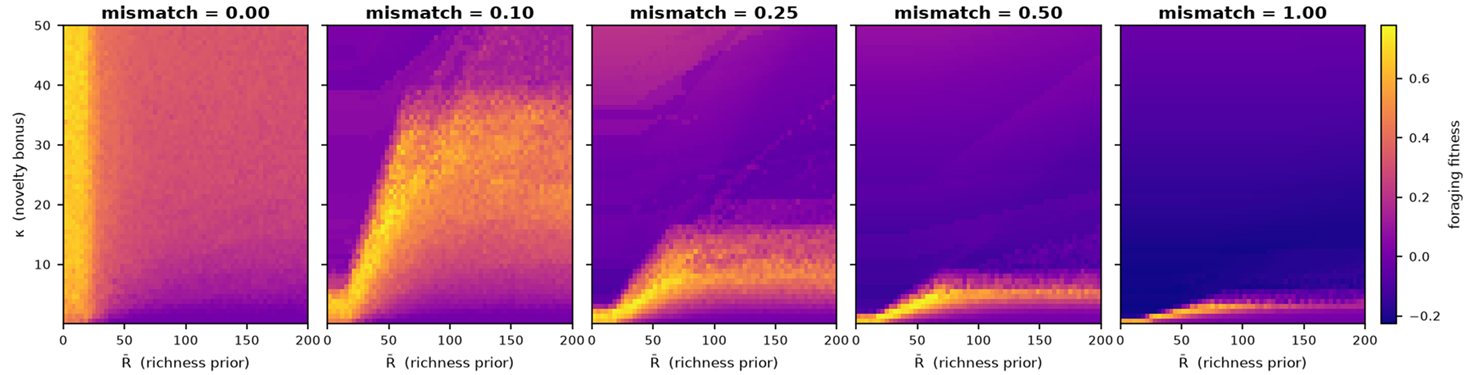
\includegraphics[height =0.16 \paperheight]{colour_plots.png} \\
    \caption{ \fontsize{29}{29}\selectfont In a honest ancestral world with \textbf{zero mismatch, curiosity is unpunished}. As novelty decouples from value and \textbf{mismatch increases, a ceiling is created on curiosity}.
    
    The variance of the expected richness for the environment increases as the marginal value theorem rule stops firing}
\end{center}
}

\begin{columns}

% First column
\column{0.33}

\block{}{
\begin{center}
    \textbf{ When does chasing novelty stop paying off? }
\end{center}
The optimum for novel information seeking depends on how correlated novelty is to value~\cite{poli2024}. As the modern world brings novel but invaluable information, \textbf{the ideal level of novelty seeking falls}. A mind adapted for chasing novelty, goes from thriving to failing as the world gets more modern while less novelty driven strategies still thrive.

\begin{center}
    \textbf{ Why internet foraging feels like compulsion? }
\end{center}
The urge to constantly forage the internet for new information is the same rule that kept us alive in an ancestral environment, running as designed. It assumes novelty is worth chasing, which held for almost all of our history. A feed breaks that assumption, so we keep trusting a signal that has started to lie.
}

\block{}{
\begin{center}
    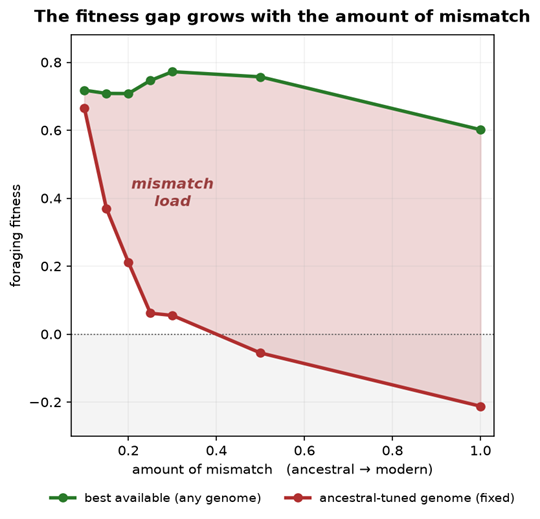
\includegraphics[height =0.18 \paperheight]{mismatch load.png} \\
    \caption{The best fitness available at each mismatch level stays high as an ancestral-tuned genome, falls below zero. The gap is the mismatch load.
}
\end{center}
}

\block{}{
\fontsize{15}{17}\selectfont
\textbf{References}\par
\begin{thebibliography}{9}
\setlength{\itemsep}{-2pt}\setlength{\parsep}{-2pt}
\bibitem{charnov1976} Charnov, E.L.\ (1976). Optimal foraging, the marginal value theorem. \textit{Theor.\ Popul.\ Biol.}\ 9, 129--136.
\bibitem{kilpatrick2020} Kilpatrick, Z.P., Davidson, J.D.\ \& El Hady, A.\ (2020). Normative theory of patch foraging decisions. \textit{arXiv}:2004.10671.
\bibitem{poli2024} Poli, F., O'Reilly, J.X., Mars, R.B.\ \& Hunnius, S.\ (2024). Curiosity and the dynamics of optimal exploration. \textit{Trends Cogn.\ Sci.}\ 28, 441--453.
\bibitem{hayden2011} Hayden, B.Y., Pearson, J.M.\ \& Platt, M.L.\ (2011). Neuronal basis of sequential foraging decisions in a patchy environment. \textit{Nat.\ Neurosci.}\ 14, 933--939.
\bibitem{kolling2012} Kolling, N., Behrens, T.E.J., Mars, R.B.\ \& Rushworth, M.F.S.\ (2012). Neural mechanisms of foraging. \textit{Science} 336, 95--98.
\end{thebibliography}
}


\column{0.67}

\block{\vspace{-1cm}\fontsize{48}{48}\selectfont The Model: A two-state neuron that forages.  \vspace{-1cm}}{
A forager has two heritable traits: $\bar{R}$ (the estimated average value of the environment) and $\kappa$ (how much novelty adds to perceived value). The forager perceives a patch's scent as its value combined with its novelty. $V$ and $\beta$ change by the ODEs below:
\begin{align*}
\frac{dV}{dt} = \frac{\scent - (V - \Vrest) - \beta}{\tauV}, \quad \frac{d\beta}{dt} = \frac{\prox\,(\bar{R} - \scent) - (1-\prox)\,\beta}{\taubeta},
\end{align*}
\begin{itemize}
    \item \quad $\scent := \val + \kappa \cdot \novelty, \quad 
\novelty := (1-m)\,(\val \times \fresh) + m$. 
    \item \quad $m$ is the mismatch variable ($0=$ ancestral, $1=$ modern), 
    \item \quad $\tauV$ and $\taubeta$ are time constants and freshness measures how much a patch has been harvested. 
    \item \quad $V$ is a leaky integrate-and-fire membrane: it integrates perceived scent and fires when it crosses threshold $\theta = -55$~mV (from rest $-65$~mV). Every spike harvests value from the patch.
    \item \quad $\beta$ is an ACC/PFC opportunity-cost signal~\cite{hayden2011,kolling2012}: while on a patch ($\prox \approx 1$) it rises by the value foregone elsewhere, $\bar{R} - \scent$, and relaxes while travelling ($\prox \approx 0$). The forager abandons a patch once $\beta$ exceeds the scent still on offer.
\end{itemize}

\quad 

In this model, an agent moves by chemotaxis: a random walk biased up the scent gradient, scaled by engagement. During a simulation, information patches appear and later disappear once fully harvested, the fitness function for the this agent is measured by the total value harvested per unit time, minus time wasted engaging patches without gaining value. The figure below shows the path of one agent acting upon a single information patch
\begin{center}
    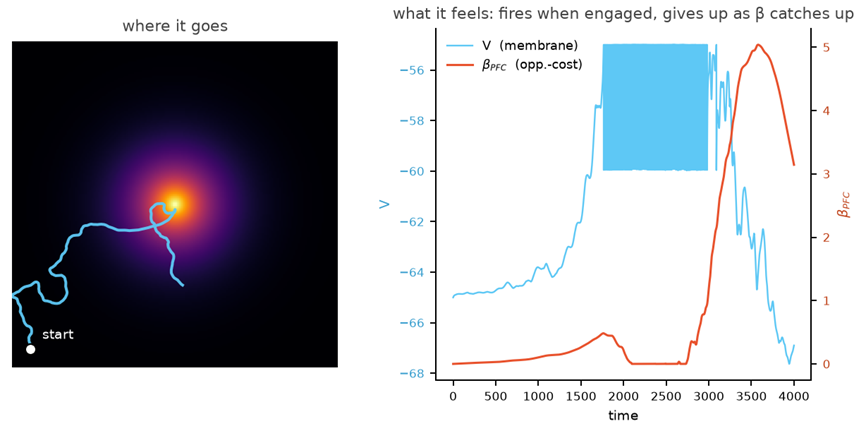
\includegraphics[height =0.12 \paperheight]{plots.png} \\
    \caption{A single run of an agent acting upon a stimulus. The agent wanders in on scent, fires while engaged, then leaves once $\beta$ is greater than the richness prior.}
\end{center}

}

\block{ \vspace{-1cm}\fontsize{48}{48}\selectfont Research Outcome: \vspace{-1cm}}{ As the modern world now has the internet and social media feeds that provide us with endless amounts of new information, minds evolved to prize novelty get trapped into over consumption. The fitness landscape for a model that shows a change into this environment shows that there still exists a strategy that could avoid being trapped by modern stimuli. The issue is that the emergence of the internet and social media feeds has come at a rate that biological evolution can't keep up with. The previously adapted genes are no longer favored in a new environment. This change in fitness landscape shows \textbf{Evolutionary Mismatch}.
}
\end{columns}
{
\colorlet{blockbodybgcolor}{white}
\colorlet{blockbodyfgcolor}{black}
\colorlet{blocktitlebgcolor}{white}
\colorlet{blocktitlefgcolor}{black}
\block{}{%
\vspace{-2.0cm}
\begin{center}
    
\includegraphics[height=0.05\paperheight]{bern.png} \quad \quad  \quad \quad  \quad \quad 
\includegraphics[height=0.04\paperheight]{Midnight black.png} \quad \quad \quad \quad   \quad\quad
\includegraphics[height=0.05\paperheight]{SURE logo (transparent background).png}
\end{center}
}
}

\end{document}

